\documentclass[final, 12pt, aspectratio=169, xcolor={dvipsnames}]{beamer}
%\usepackage[table]{xcolor}
\usepackage{lmodern}
\usepackage[utf8]{inputenc}
\usepackage[T1]{fontenc}
\usepackage{graphicx} 
\usepackage{textpos} % package for the positioning
\usepackage{xcolor}
\usepackage{tcolorbox}
\usepackage{tabularx}
\usepackage{hanging}
\usepackage{animate}
\usepackage{caption}
\usepackage{xcolor}

\title[PEARL]{The long-term effects of national residential planning policy: the case of VINEX}
\subtitle[PEARL]{}
\author[T. Husby]{Trond Grytli Husby (PBL), Christian Lennartz (PBL), Wolter Hassink (UU)}
\institute[PBL]{
  ODISSEI Community Conference \\[5ex]
  \texttt{trond.husby@pbl.nl}
}
\date[\today]{24 November, 2020}

% set path to figures
\newcommand*{\figs}{../figs}%

% position the logo
\addtobeamertemplate{background}{}{%
  %\begin{textblock*}{100mm}(0.95\textwidth, 7cm)
  %\begin{flushright}
    
\includegraphics[width=\paperwidth, height=\paperheight]{\figs/pbl_background.pdf}
  %\end{flushright}
    %\end{textblock*}}
}

% colour scheme and settings
\setbeamercolor{title}{bg=white,fg=blue!35!black}
\setbeamercolor{frametitle}{bg=,fg=PineGreen}
\setbeamercolor{enumerate item}{fg=PineGreen}
\setbeamercolor{itemize item}{fg=PineGreen}
\setbeamertemplate{itemize item}[circle]
\setbeamercolor{itemize subitem}{fg=PineGreen}
\setbeamertemplate{itemize subitem}[triangle]
\setbeamerfont{frametitle}{size=\normalsize}
\addtobeamertemplate{frametitle}{\vspace*{1cm}}{\vspace*{0.0cm}}
\setbeamertemplate{footnote}{\hangpara{2em}{1}\makebox[2em][l]{\insertfootnotemark}\footnotesize\insertfootnotetext\par}

% miscellaneous
\newcommand{\semitransp}[2][35]{\color{fg!#1}#2}
\newcommand{\source}[1]{\caption*{\tiny Source: {#1}} }


\begin{document}

\beamertemplatenavigationsymbolsempty

%--- the titlepage frame -------------------------%
{
  \setbeamertemplate{footline}{}

  \begin{frame}
    \titlepage
  \end{frame}
}


%---  --------------------------------%
\begin{frame}{Background \footnote{Van der Wouden (2015). "De ruimtelijke metamorfose \newline van Nederland 1988–2015." }}
  \begin{minipage}{0.48\linewidth}%
    \small
    \begin{itemize}
    \item VINEX (1995 - 2005): supplement to the Fourth National Policy Document on Spatial Planning
    \item Goals: create living environment with high level of urban amenities, reduce mobility and protect nearby rural areas $\rightarrow$ compact city
    \item Vinex locations: large-scale residential development projects (mostly) on the urban fringe
      \end{itemize}
    \end{minipage}
  %\hfill%
  \begin{minipage}{0.48\linewidth}%
    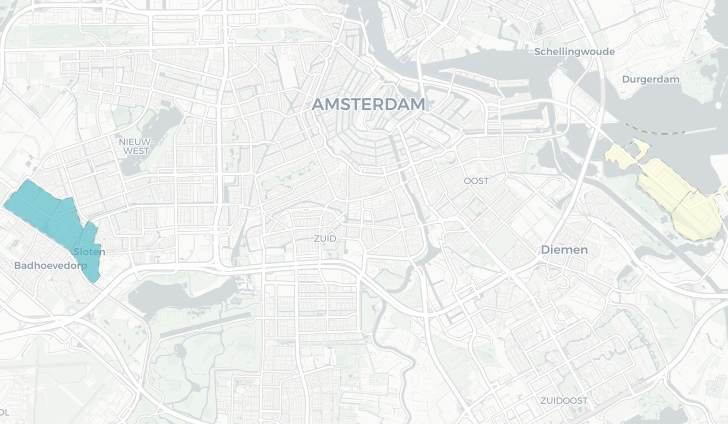
\includegraphics[scale = 0.3]{\figs/vinex_locations_adam.png}
    \end{minipage}
  \end{frame}

\begin{frame}{Research question and design}
  \begin{minipage}{0.58\linewidth}%
    \begin{itemize}
    \item What were the long-term effects of Vinex? Were the goals of less commuting and high quality housing achieved?
     \item Focus on buyers of newly built dwellings
      \item Variables of primary interest: commuting distance and estimated home value
      \item Difference in difference design
        \begin{itemize}
        \item Treatment: moved to a Vinex neighbourhood
          \item Control: moved to a non-Vinex neighbourhood
          \end{itemize}
      \end{itemize}
  \end{minipage}
  \hfill%
  \begin{minipage}{0.38\linewidth}%
    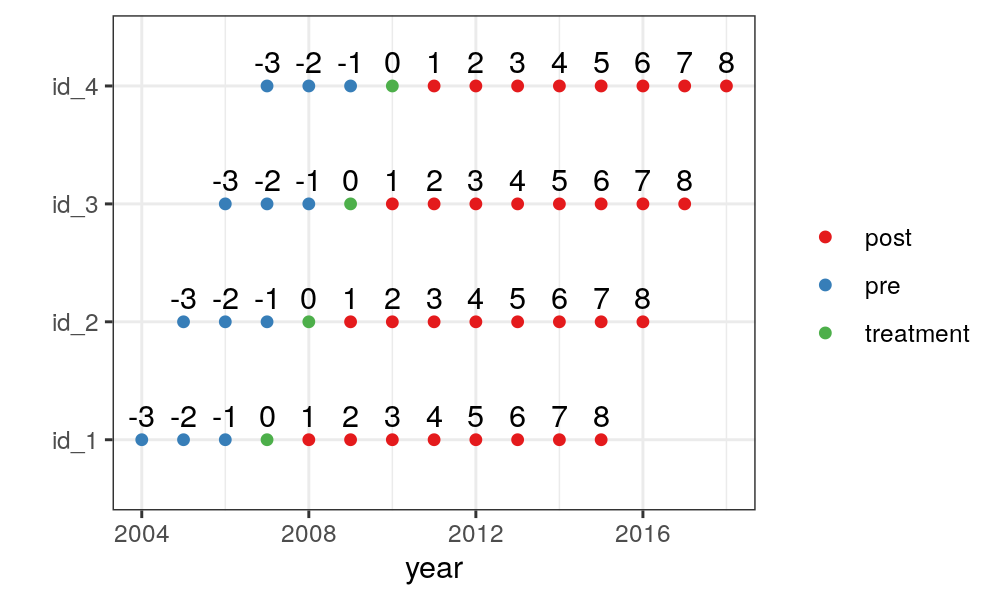
\includegraphics[scale = 0.5]{\figs/did_selection.png}
    \end{minipage}
\end{frame}


\begin{frame}{Data and OSSC}
  \begin{itemize}
  \item We use a range of municipal registry data (address, person, household)...
  \item ...coupled with building registry data..
  \item ...and data on monthly employment status and location of work municipality
  \item OSSC: create basic data set of all address changes of every person in the Netherlands between 1995 - 2018, find household number and members around date of move
  \item Pilot project: tried out new software (Apache Spark), monitored performance, compared timings between OSSC and RA
  \end{itemize}

\end{frame}

\begin{frame}{Why OSSC?}
  \end{frame}

\begin{frame}{Action shot of an R-user during a session with the normal RA}
  \centering
  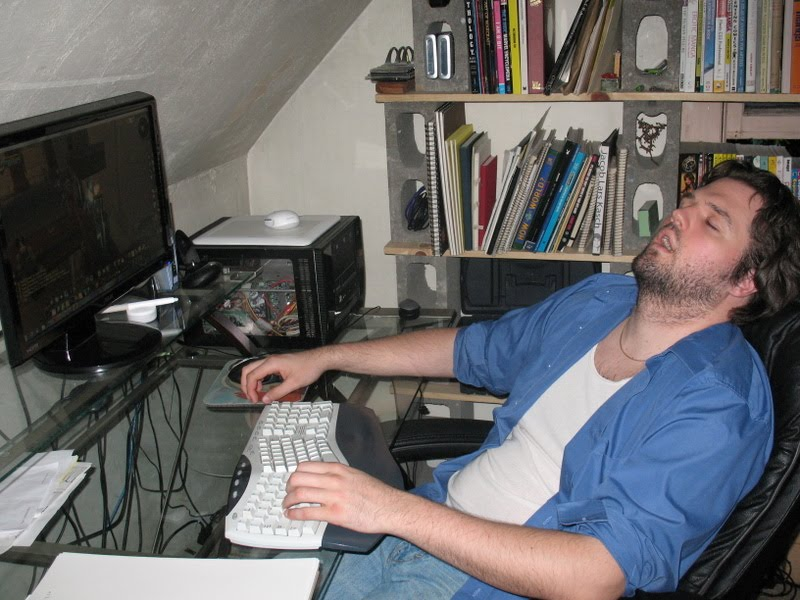
\includegraphics[scale = 0.3]{\figs/falling_asleep.jpg}
  \\
  \tiny
  \url{https://www.unibetcommunity.com/t5/image/serverpage/image-id/21516i0C3F0F5C000AA38F/image-size/large?v=1.0&px=999}
  \end{frame}

\begin{frame}{Summary statistics, time period 0}
% latex table generated in R 3.6.3 by xtable 1.8-4 package
  % Fri Nov 20 14:40:59 2020
  \vspace{-0.7cm}
\begin{table}[ht]
\centering
\begin{tabular}{lllll}
  \hline
 & Control &  & Treatment &  \\ 
  \hline
 & mean & sd & mean & sd \\ 
  single family home & 	\textcolor{blue}{0.62} & 0.49 & 	\textcolor{red}{0.79} & 0.4 \\ 
  m2 & 	\textcolor{red}{168.27} & 626.19 & 	\textcolor{blue}{154.96} & 287.41 \\ 
  age & 	\textcolor{red}{42.38} & 12.8 & 	\textcolor{blue}{38.46} & 10.88 \\ 
  household size & 	\textcolor{blue}{2.42} & 1.33 & 	\textcolor{red}{2.55} & 1.74 \\ 
  spouse & 	\textcolor{red}{0.61} & 0.49 & 	\textcolor{blue}{0.6} & 0.49 \\ 
  dutch & 	\textcolor{red}{0.92} & 0.27 & 	\textcolor{blue}{0.89} & 0.31 \\ 
  children & 	\textcolor{blue}{0.27} & 0.45 & 	\textcolor{red}{0.36} & 0.48 \\ 
  density & 	\textcolor{red}{1623.52} & 1455.85 & 	\textcolor{blue}{1307.46} & 440.36 \\
    distance to agglommeration (centre) & 	\textcolor{red}{16.36} & 13.15 & 	\textcolor{blue}{9.53} & 6.3 \\ 
  move distance & 	\textcolor{blue}{11.19} & 25.32 & 	\textcolor{red}{12.1} & 22.47 \\ 
  N & 59473 &  & 24423 &  \\ 
   \hline
\end{tabular}
\end{table}  
\end{frame}

\begin{frame}{Mean of dependent variables}
  \centering
  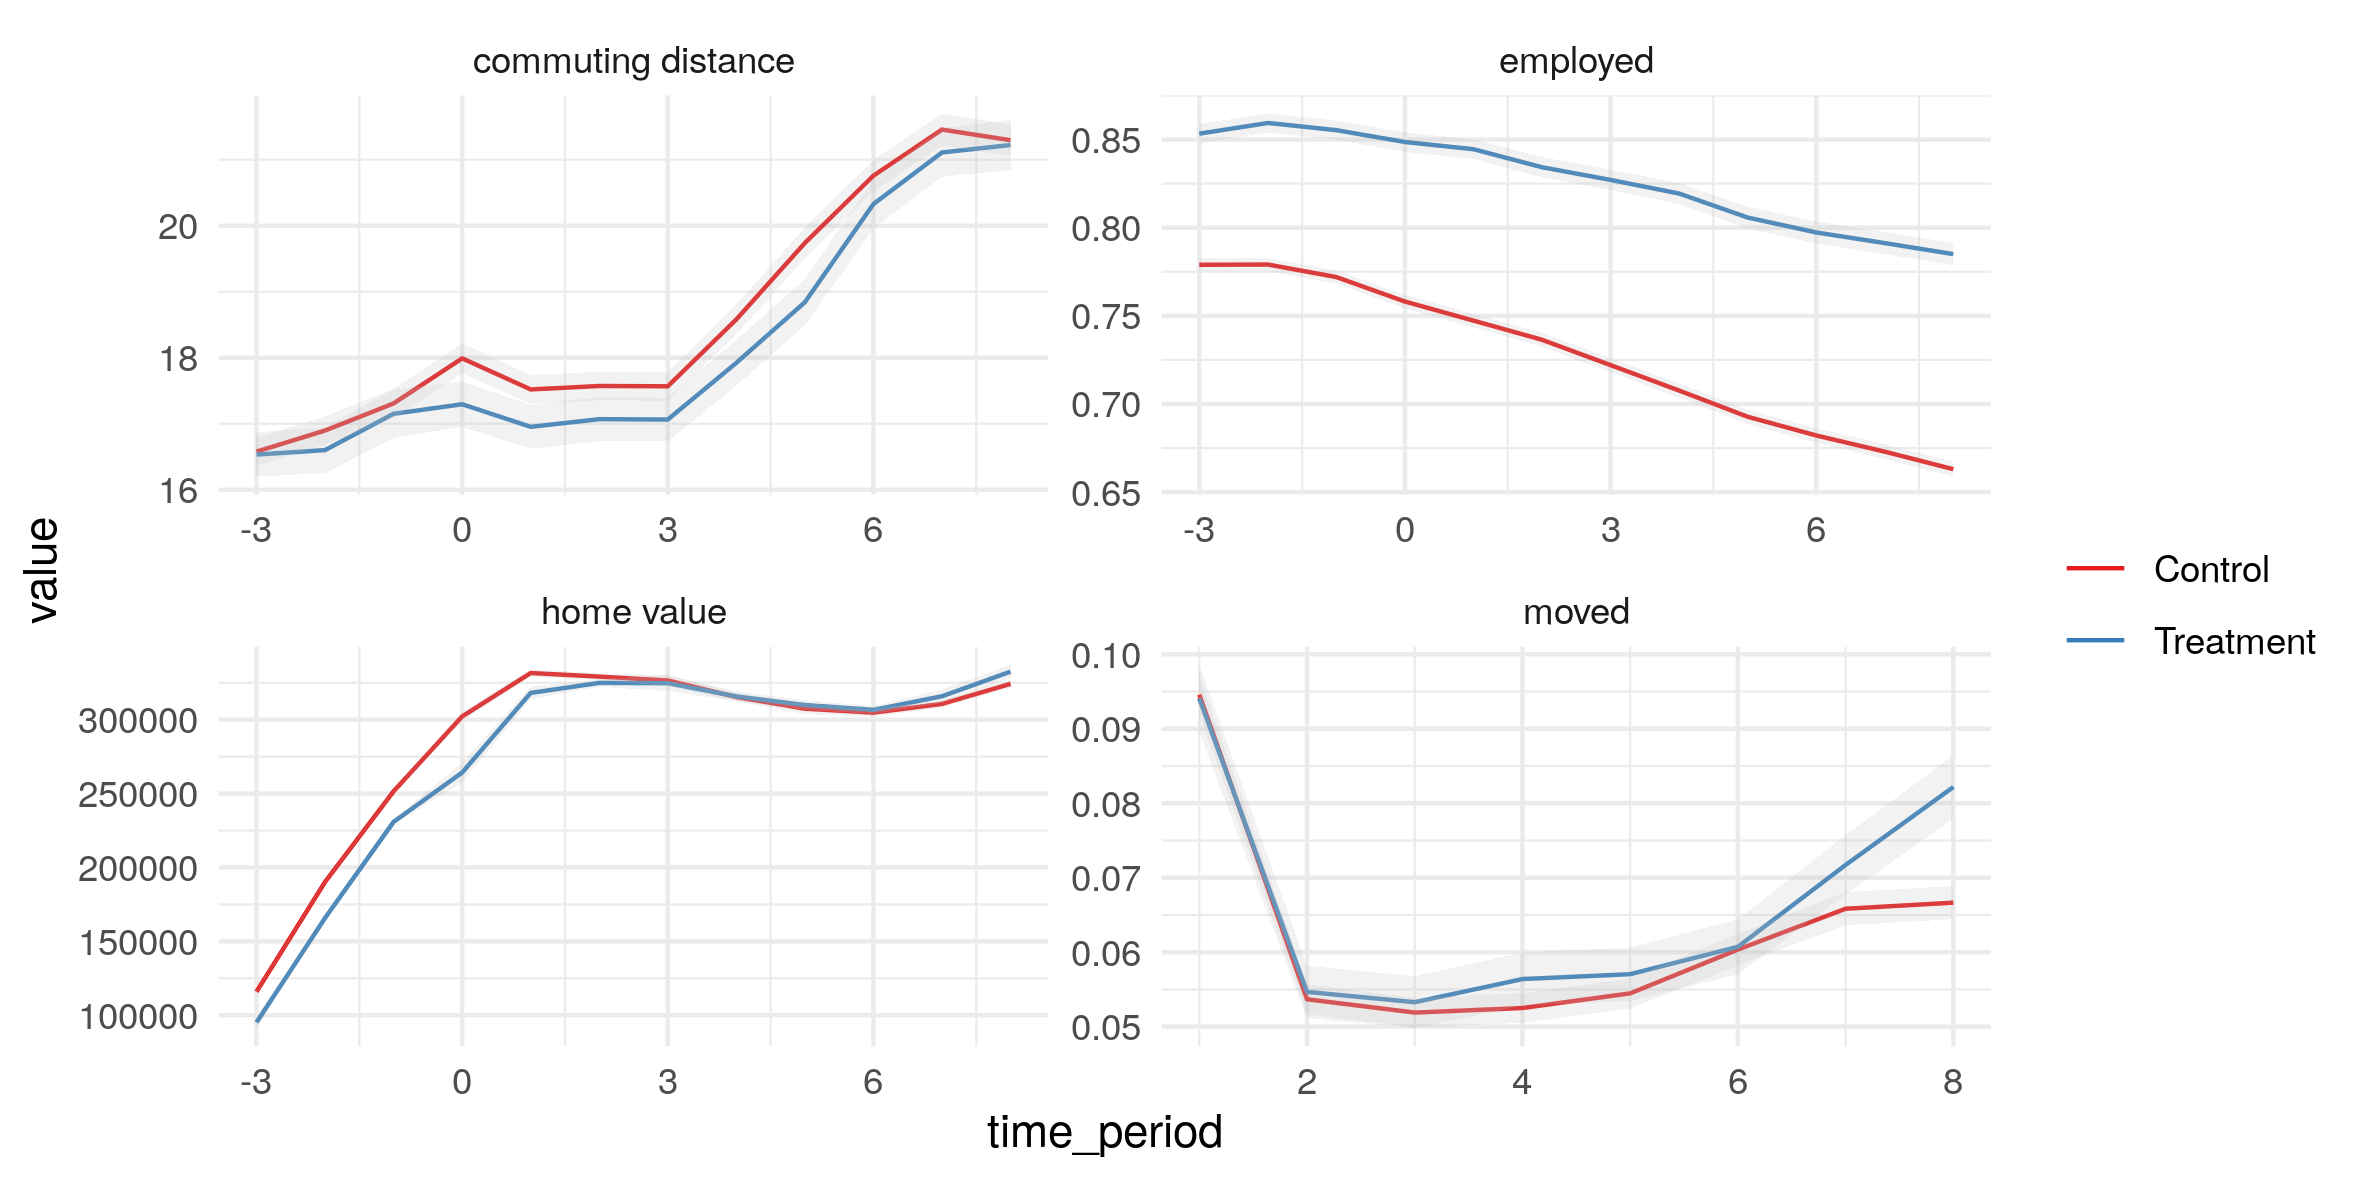
\includegraphics[scale = 0.6]{\figs/dep_vars.png}
 \end{frame}


\begin{frame}{Conclusions and further work}
  \begin{itemize}
  \item Work in progress: refine identification strategy, matching on individual, dwelling and regional level
    \item OSSC: used interactively for computations that could have been done on RA (but would have been much slower) 
  \item Many quirks from the Pilot environment have been removed
  \item Less developed than AWS or Azure, compensated with good user support
    \item Still a fairly steep learning curve. My two cents: either improve communication between OSSC and RA, or invest in user-friendly interface of OSSC
    \end{itemize}
\end{frame}

\end{document}






